\documentclass[letter,12pt, usenames,dvipsnames]{article}

\usepackage{verbatim}
\usepackage{enumerate}
\usepackage{amsmath}
\usepackage{multicol}
\usepackage{graphicx}
\usepackage{hyperref}
\usepackage{tikz}
\usetikzlibrary{arrows,automata}
\usetikzlibrary{positioning}
\usetikzlibrary{shapes}
\usetikzlibrary{shapes.geometric,backgrounds, arrows, positioning}
\usetikzlibrary{arrows, decorations.markings}

\usepackage{fullpage}

\newcommand{\MYhref}[3][Blue]{\href{#2}{\color{#1}{#3}}}
\newcommand{\hash}{\#}
\newcommand{\underscore}{\_}


%****************
% Tikz Nodes
\tikzset{human node/.style={draw=black, very thick,rectangle, rounded corners, minimum height=1.5cm, minimum width=2cm, text width=2cm, align=center,  fill=black!40}}
\tikzset{nonhuman node/.style={draw=black, very thick, rectangle,  rounded corners, minimum height=1.5cm, minimum width=2cm, text width=2cm, align=center, fill=NavyBlue!20}}
\tikzset{modelComponent node/.style={draw=black, very thick, rectangle,  rounded corners, minimum height=3cm, minimum width=4cm, text width=3cm, align=center, fill=NavyBlue!20}}

%NavyBlue!20

\tikzset{normalArrow/.style={->, line width=1mm}}
\tikzset{changedArrow/.style={->, line width=1mm, BrickRed}}
\tikzset{normalDashedArrow/.style={->, dotted, line width=1mm}}
\tikzset{changedDashedArrow/.style={->, dotted, line width=1mm, BrickRed}}
% End Tikz Nodes
%****************

\definecolor{myhighlight}{rgb}{0.858, 0.188, 0.478}

\begin{document}

\vfill
\title{UN-OCHA Infectious Disease Modelling Final Report}
\author{Shelby N. Wilson, Ph.D., Michael Kelbaugh, Jason A. Lee} 
\date{February 2021}

\maketitle

\vfill
\begin{center}
{\Large
THE JOHNS HOPKINS UNIVERSITY APPLIED PHYSICS LABORATORY (JHU/APL) \\ {\it written for}\\[1.3ex] THE UNITED NATIONS OFFICE FOR THE COORDINATION OF HUMANITARIAN AFFAIRS (UN OCHA) CENTRE FOR HUMANITARIAN DATA
}
\end{center}
Document \hash AOS-21-0261
\pagebreak
 

\section{Overview} 
\subsection{Statement of Work} 
The collaboration between JHU/APL and the UN OCHA Centre for Humanitarian Data has provided research, support, and development of models to inform humanitarian intervention strategies by both governments and the humanitarian community. In 2020, this work primarily focused on the effects of COVID-19 and the development of the OCHA-Bucky model. Documentation on data requirements, approach, and standard operating procedures, including training materials, for the OCHA-Bucky model has previously been provided by JHU/APL to UN OCHA over the course of this effort; appropriate documentation for these tasks may be found \MYhref{https://data.humdata.org/dataset/2048a947-5714-4220-905b-e662cbcd14c8/resource/2d9592f8-2980-4466-96f5-f0de23ea7ffa/download/ochabucky_final.pdf}{here} and \MYHref{https://ocha-bucky.readthedocs.io/en/latest/}{here}.

While modelling COVID-19 in humanitarian regions remains a priority for OCHA country offices, partner organisations, and ministries of health, the immediate impacts of the COVID-19 crisis may manifest themselves indirectly in plans and actions for other infectious diseases.  As such, this document details the procedures that may be taken to model other infectious diseases that may be impacted by interventions put into place during the course of the COVID-19 pandemic.  For this effort, we will focus on cholera, malaria, and measles as use cases. These diseases are most prevalent in humanitarian regions of interest, and most related to, and therefore directly impacted by, the mitigation efforts put into place during the COVID-19 pandemic. 

Models presented herein are three variants on the classic SIR model \cite{basicSIR} where each disease and each geographic region are parameterized independently. In addition to a baseline set of parameters, designed to most closely align with historical data, each model is also designed as a simulation tool wherein different scenarios that might effect disease spread can be run. Scenarios are recommended to include a worst case, best case, and ``business as usual" scenario which should be considered the most likely given the current situation as described by the data and inputs from country offices and stakeholders.   Each of these models is designed to give insight into the mid-term effects of characteristics associated with disease spread as well as the distribution of effects that might be observed in the presence of extra-ordinary circumstances (e.g., COVID-19 pandemic, flooding, large infusion of resources, etc.).
 




\section{Workflow and Methodology}

\subsection{SIR Models}
\label{sec:SIR}
The SIR model framework is one of the most widely used modeling techniques for considering community spread of infectious diseases \cite{basicSIR}.  Disease dynamics are modelled over time by probabilistically moving individual members of the population through a series of compartments (otherwise known as "bins" or "states").  Those states are as follows:
\begin{itemize}
    \item Susceptible (S): the fraction of the population that could be potentially subjected to the infection;
    \item Exposed (E): the fraction of the population that has been infected but does not show symptoms yet;
    \item Infectious (I): the fraction of the population that is infective after the latent period;
    \item Recovered (R): the fraction of the population that has been infected and recovered from the infection.\\
\end{itemize}

\noindent The total population is represented by the sum of the compartments.  Basic assumptions of this type of model include: 
\begin{itemize}
    \item Once the model is initialized, no individuals are added to the susceptible group.  It follows that births and natural deaths are unaccounted for, migration into and out of the region is frozen for the duration of a simulation, and none of the population has been vaccinated or is immune to the pathogen;
    \item The population within each strata is uniform, and each pair of individuals within the strata are equally likely to interact;
    \item The probability of interaction between individuals in the population is not rare;
    \item Once infected, an individual cannot be reinfected with the virus; 
	\item Models for each disease are developed independently, and joint effects between models of multiple diseases are not considered.
\end{itemize}

The infectious diseases chosen, along with the geographic scale on which they are modelled, meet the conditions described above and therefore qualify as candidates to be modeled in this way.  We have considered the body of literature related to modelling cholera, malaria, and measles and have chosen three candidate models as a base on which to build our sub-national infectious disease models.  Details for the cholera model are given in Section \ref{sec:cholera};  details for the malaria model are given in Section \ref{sec:Malaria}; and details for the measles model are given in Section \ref{sec:Measles}.

Somalia is the use-case for which we have developed each of these models.  Baseline models, are presented in Section \ref{sec:Simulations}.  The goal of this work is to use this framework as the first steps towards the creation of a ``scenario modelling environment" in which decision makers can model the effects of a number of different public health outcomes depending on current and future plans. A summary of the general framework, as well as the external factors that might lead to the need for planning scenario building within the model are given in Figure \ref{fig:basicFramework}. 
\begin{figure}[h!]
\centering
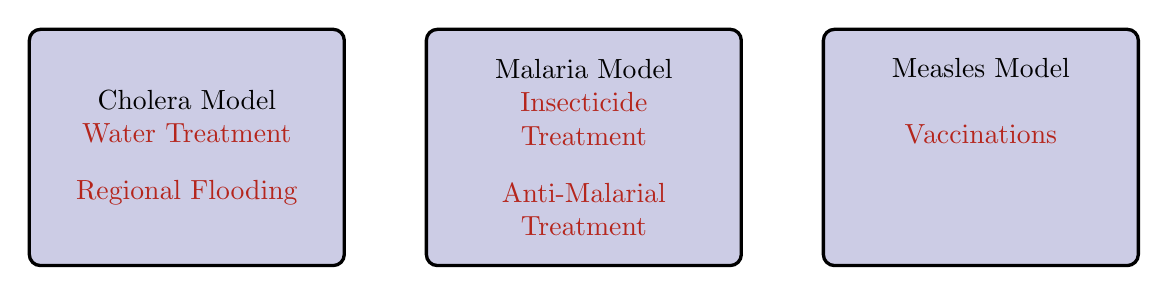
\begin{tikzpicture}

  \node[modelComponent node] (cholera) {Cholera Model\\{\color{BrickRed} Water Treatment\\[2ex]Regional Flooding}};
  \node[modelComponent node, right=1cm of cholera] (malaria) {Malaria Model\\{\color{BrickRed} Insecticide Treatment\\[2ex] Anti-Malarial Treatment}};
  \node[modelComponent node, right=1cm of malaria] (measles) {Measles Model\\~\\{\color{BrickRed} Vaccinations}\\[5ex]~};
\end{tikzpicture}

\caption{The current modelling framework includes independent, sub-national models for cholera, malaria, and measles.  For each model, in red, examples are provided (in red) as to the types of factors that might contribute to generating planning scenarios to support decision making.}

\label{fig:basicFramework}
\end{figure}

\subsection{Model Selection}
A number of models were reviewed and evaluated for their potential to be used in this task.  A listing of evaluated models can be found in the Appendix, Section \ref{sec:Appendix}. Final models were selected based on a number of criteria, including, but not limited to: 

\begin{itemize}
    \item the number of citations the model has;
    \item the thoroughness of the documentation included in the manuscript;
    \item the ability of the model to be parameterized to real world data; and
    \item the amenability of the model to parameter adjustments for the purposes of building scenarios.
\end{itemize}

\subsection{Model Parameterization and Implementation}
\label{sec:Parameterization}
Each model is currently implemented in Python Version 3.8 with code and associated documentation provided by JHU/APL.

Model parameterization is performed via a least squares fit (performed via the python function \textit{``Fit"} contained in the \textit{symfit} library of python).  The quantity being minimized is the difference between model output and available data regarding the percentage of infected individuals in a geographical region at the given time points.


\section{Models}
\subsection{Cholera}
\label{sec:cholera}
\subsubsection{Model Overview}
Literature is rich with various mathematical models of cholera.  For this task, we have chosen the model developed in {
\MYhref{https://www.ncbi.nlm.nih.gov/pmc/articles/PMC6676578/pdf/13104_2019_Article_4504.pdf}{Nyabadza et al}} \cite{cholera}.  The following documentation explains the developed cholera model and draws heavily from \cite{cholera}.

Presented here is a compartmental deterministic
mathematical model with a suitable treatment function
in order to study the impact of limited hospital resource
capacity on Cholera disease. The number of available
hospital beds per 10,000 (hospital bed:population ratio)
is used by health planners as a method of estimating
resource availability to the public. This model incorporates a disease recovery rate that is a function of the capacity of the health care system in terms of hospital bed-population ratio.

\subsubsection{Cholera Background}
 Cholera is an acute gastro-intestinal infection and waterborne disease which is caused by the bacterium \textit{Vibrio
Cholerae}, \textit{V. cholerae} O1 or O139. Bacterial cholera infection induces vomiting and diarrhea, and when patients are treated with delay, it can lead to severe dehydration and death within few hours. The disease has two modes
of transmission: direct transmission (human–human), which is very uncommon, and indirect transmission (environment–human), which occurs by a human ingesting contaminated food or water.

An estimated $100,000 - 120,000$ deaths are due to cholera every year in the world with only a small proportion being reported to World Health Organization (WHO).


\subsubsection{Modelling Cholera}
A diagram displaying the components of the Nyabadza cholera model is given in Figure \ref{fig:CholeraDiagram}.  The corresponding system of equations is given by Equation System (\ref{eqn:choleraEquations}).  Descriptions of the variables and parameters are given in Tables \ref{table:CholeraVariables} and \ref{table:CholeraParameters} respectively.

\begin{figure}[h!]
\centering
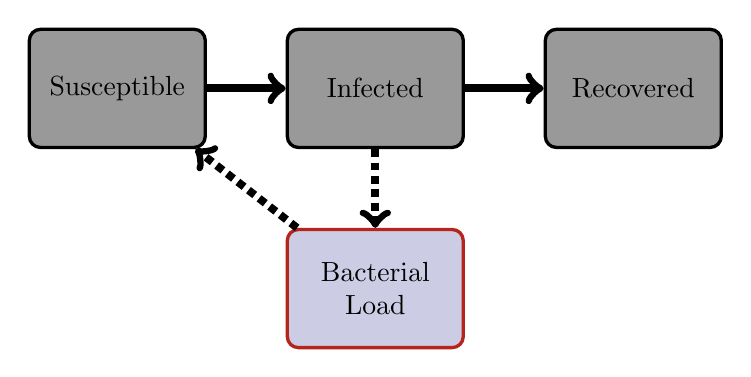
\begin{tikzpicture}
  \node[human node] (susceptible) {Susceptible};
  \node[human node, right=of susceptible] (infected) {Infected};
  \node[human node,right=of infected] (recovered) {Recovered};
  \node[nonhuman node, below=of infected, draw=BrickRed,very thick] (bacteria) {Bacterial Load};
  
  % the edges
   \draw[normalArrow] (susceptible) -> (infected);
   \draw[normalArrow] (infected)-> (recovered) ;
   \draw[normalDashedArrow] (infected)-> (bacteria);
   \draw[normalDashedArrow] (bacteria)-> (susceptible);
\end{tikzpicture}

{\color{BrickRed}Water Treatment}

\caption{Model diagram for the cholera model.  Model details are given in \cite{cholera}. Compartments that represent humans are grey in color.  Compartments that represent transmission mechanisms (bacteria) are blue in color.  Solid black lines represent the flow between similar species compartments, while dashed arrows represent points of interactions between humans and vectors. Red indicates a factor that can be changed to build scenarios.}
\label{fig:CholeraDiagram}
\end{figure}


\begin{align}
\label{eqn:choleraEquations}
\begin{split}
\frac{dS}{dt} &= \mu N - \beta_1 \frac{SI}{N}-\beta_2\frac{SB}{B+k} - \mu S,\\
\frac{dI}{dt} &= \beta_1\frac{SI}{N} +\beta_2\frac{SB}{B+k} - \gamma (b,I)I - \mu I,\\
\frac{dR}{dt} &= \gamma (b,I)I - \mu R,\\
\frac{dB}{dt} &= \alpha I - \delta B.\\
\end{split}
\end{align}

The cholera model developed by Nyabadza, et al. classifies the human population at
time $t$, denoted by $N(t)$, into susceptible individuals $S(t)$,
cholera infected individuals $I(t)$ and recovered individuals $R(t)$, such that: $$N(t) = S(t) + I(t) + R(t)$$ 
An additional compartment $B(t)$, representing the concentration of \textit{V. cholerae} in contaminated water has also been  incorporated in the model. Further description of the variables given in System (\ref{eqn:choleraEquations}) are defined in Table \ref{table:CholeraVariables}.

\begin{table}[h!]
\centering
\begin{tabular}{|l|l|}
\hline
Variable & Description \\\hline\hline 
$N(t)$ & Total population\\\hline
$S(t)$ & Susceptible individuals \\\hline
$I(t)$ & Infected individuals \\\hline
$R(t)$ & Recovered individuals\\\hline
$B(t)$ & Bacterial levels in water\\\hline
$\gamma (b, I)$ & Recovery rate of individuals\\\hline
\end{tabular}
\caption{Variable labels for the Nyabadza cholera model.  Further details about initial conditions and parameter values used can be found in the APL-provided code.  Further details about the model structure and analysis can be found in \cite{cholera}.}
\label{table:CholeraVariables}
\end{table}

\begin{table}[h!]
\centering
\begin{tabular}{|l|l|}
\hline
Parameter & Description \\\hline\hline 
$\mu$ & Natural death rate of humans\\\hline
$\beta_1$ & Effective contact rate between individuals \\\hline
$\beta_2$ & Per capita contact rate for humans and the
contaminated environment\\\hline
$\hat{k}$ & Half-saturation constant\\\hline
$\gamma_0$ & Minimum recovery rate of human\\\hline
$\gamma_1$ & Maximum recovery rate of human\\\hline
$\hat{b}$ & Hospital bed-population ratio\\\hline
$\delta$ & Bacterial net death rate\\\hline
$\alpha$ & Shedding rate\\\hline
\end{tabular}
\caption{Parameter descriptions for the Nyabadza cholera model.  Further details about initial conditions and parameter values used can be found in the APL-provided code.  Further details about the model structure and analysis can be found in \cite{cholera}.}
\label{table:CholeraParameters}
\end{table}

\pagebreak
\subsection{Malaria} 
\label{sec:Malaria}
\subsubsection{Model Overview}
Malaria is well studied both in terms of biology as well as associated models of the disease processes.  For this task, we have chosen the model developed in {\MYhref{http://streaming.ictp.it/preprints/P/99/158.pdf}{Ngwa and Shu}} \cite{malaria}.  The following documentation explains the aforementioned model and draws heavily from \cite{malaria}.


In \cite{malaria}, a deterministic differential equation model for endemic malaria involving variable human and mosquito populations is presented. Humans are modeled using an SEIR model, while mosquitoes are modeled via an SIR model.




\subsubsection{Malaria Background}
 Malaria is a parasitic vector borne disease endemic in many parts of the world.  At present, at least 300 million people are affected worldwide, and there are between 1-1.5 million malaria related deaths annually. The endemicity and prevalence of malaria varies within and between countries due to environmental factors such as climate, rainfall, and mosquito population, as well as resistance of malaria parasites to anti-malarial drugs. Malaria is caused by a protozoan parasite of the genus \textit{Plasmodium}. The parasites are transmitted from person to person by a mosquito, of the genus \textit{Anopheles}, each time the infected insect takes a blood meal. On average the incubation period of \textit{P. falciparum} is about 12 days in humans and about 10 days in mosquitoes. 

\pagebreak 

\subsubsection{Modeling Malaria}

A diagram displaying the components of the Ngwa malaria model is given in Figure \ref{fig:MalariaDiagram}.  The corresponding system of equations is given by Equation System (\ref{eqn:malariaEquations}).  

The Ngwa malaria model, System (\ref{eqn:malariaEquations}) contains human and vector populations that are divided into classes or states containing susceptible, incubating, infectious and immune individuals. At time $t$, there are $S_h$ susceptible humans, $E_h$ incubating humans, $I_h$ infectious humans, $R_h$ immune humans, $S_v$ susceptible mosquitoes, $E_v$ incubating mosquitoes and $I_v$
 infectious mosquitoes. The mosquito population does not have
an immune class since their infective period ends with their death. 
$$Nh = S_h + E_h + I_h + R_h
\text{\hspace*{.2in} and \hspace*{.2in}}
N_v = S+v + E_v + I_v$$

\noindent are respectively the total human and vector populations at time $t$. The
model assumes all newborns are susceptible in both populations and a
uniform birth rate. The per capita birth rates for humans and mosquitoes are $\lambda_h$ and $\lambda_v$ respectively. Immune human individuals loose their immunity at a rate $\beta_h$. Incubating individuals in both populations become infectious with rates $\nu_h$ and $\nu_v$. Infectious human individuals either recover without any substantial gain in immunity at rate $r_h$, or join the susceptible class or with rate $\alpha_h$ signifying a period of immunity before joining the susceptible class. All individuals in both human and mosquito populations experience per capita death rates of $f_h(N_h)$, $f_v(N_v)$ respectively and infected human individuals die from the disease at the additional rate $\gamma_h$.  Descriptions of the variables and parameters associated with System (\ref{eqn:malariaEquations}) are given in Tables \ref{table:MalariaVariables} and \ref{table:MalariaParameters} respectively.

\begin{figure}
\centering
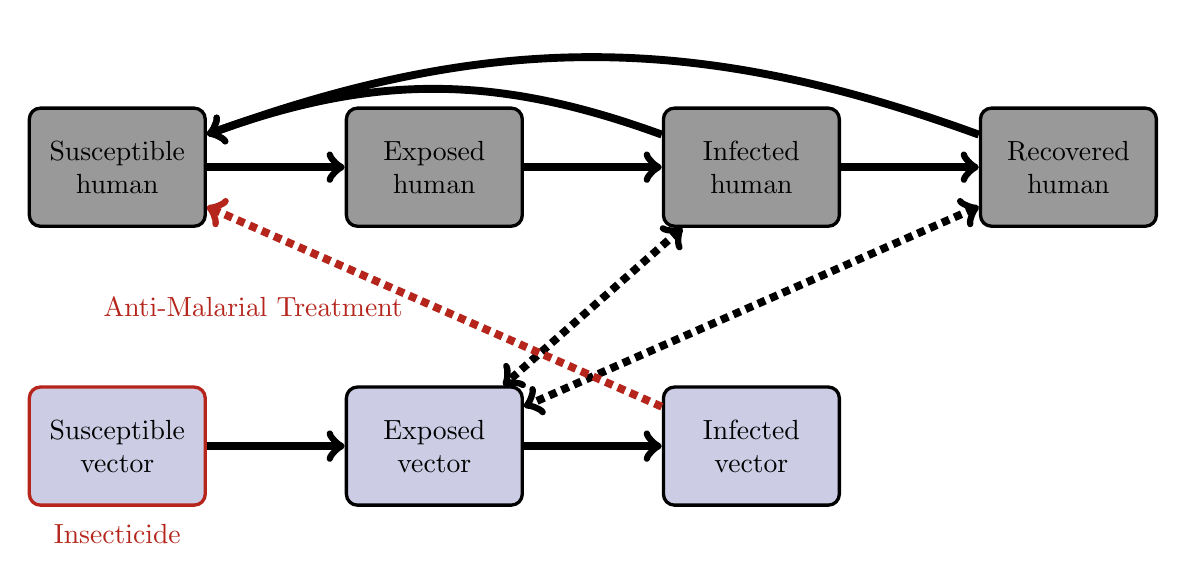
\begin{tikzpicture}
  \node[human node] (susceptible) {Susceptible human};
  \node[human node, right=1.75cm of susceptible] (exposed) {Exposed human};
  \node[human node, right=1.75cm of exposed] (infected) {Infected human};
  \node[human node, right=1.75cm of infected] (recovered) {Recovered human};
  
  \node[nonhuman node, draw=BrickRed, very thick, below=2cm of susceptible] (susceptiblev) {Susceptible vector};
  \node[nonhuman node,  below=2cm of exposed] (exposedv) {Exposed vector};
  \node[nonhuman node,  below=2cm of infected] (infectedv) {Infected vector};
  \node[below= 0.1cm of susceptiblev](Insecticide) {\color{BrickRed}Insecticide};

  
  % the edges
   \draw[normalArrow] (susceptible) -> (exposed);
    \draw[normalArrow] (exposed) -> (infected);
   \draw[normalArrow] (infected)-> (recovered) ;   
   
   \draw[normalArrow] (susceptiblev) -> (exposedv);
    \draw[normalArrow] (exposedv) -> (infectedv);

   
   \draw[normalDashedArrow, <->] (infected) -> (exposedv);
   \draw[normalDashedArrow, <->] (recovered) -> (exposedv);
   \draw[changedDashedArrow] (infectedv) -> (susceptible) 
   	node[midway, left]{Anti-Malarial Treatment~~  };
   
\draw[normalArrow] (recovered)  to [out=160,in=20] (susceptible);
\draw[normalArrow] (infected)  to [out=160,in=20] (susceptible);   
\end{tikzpicture}

\caption{Model diagram for the Ngwa malaria model.  Model details are given in \cite{malaria}. Compartments that represent humans are grey in color.  Compartments that represent vectors (mosquitoes) are blue in color.  Solid black lines represent the flow between similar species compartments, while dashed arrows represent points of interactions between humans and vectors. Red indicates a factor that can be changed to build scenarios.}

\label{fig:MalariaDiagram}
\end{figure}


\begin{align}
\label{eqn:malariaEquations}
\begin{split}
\frac{dS_h}{dt} &= \lambda_h N_h +\beta_h R_h + r_h I_h - f_h(N_h)S_h -\left(\frac{c_{vh}a_vI_v}{N_h}\right)S_h,\\
\frac{dE_h}{dt}&= \left(\frac{c_{vh}a_vI_v}{N_h}\right)S_h - (\nu_h + f_h(N_h))E_h,\\
\frac{dI_h}{dt}&= \nu_hE_h - (r_h + \alpha_h + \gamma_h + f_h(N_h))I_h,\\
\frac{dR_h}{dt}&= \alpha_hI_h - (\beta_h + f_h(N_h))R_h,\\\\
\frac{dS_v}{dt} &= \lambda_vN_v - f_v(N_v)S_v - \left(\frac{c_{vh}a_vI_h}{N_h}S_v\right) - \left(\frac{c_{vh}a_vR_h}{N_h}\right)S_v,\\
\frac{dE_v}{dt}&= \left(\frac{c_{vh}a_vI_h}{N_h}\right)S_v + \left(\frac{c_{vh}a_vR_h}{N_h}\right)S_v - (\nu_v + f_v(N_v))E_v,\\
\frac{dI_v}{dt}&= \nu_vE_v - f_v(N_v)I_v
\end{split}
\end{align}

\begin{table}[h!]
\centering
\begin{tabular}{| l | l |}
\hline
Variable & Description \\\hline\hline 
$S_h(t)$ & Susceptible  humans\\\hline
$E_h(t)$ & Exposed humans\\\hline
$I_h(t)$ & Infected humans\\\hline
$R_h(t)$ & Recovered  individuals\\\hline
$S_v(t)$ & Susceptible  mosquitoes\\\hline
$E_v(t)$ & Exposed  mosquitoes\\\hline
$I_v(t)$ & Infected mosquitoes\\ \hline
\end{tabular}
\caption{Variable descriptions for the Ngwa malaria model.  Further details about initial conditions and parameter values used can be found in the APL-provided code.  Further details about the model structure and analysis can be found in \cite{malaria}.}
\label{table:MalariaVariables}
\end{table}

\begin{table}[h!]
\centering
\begin{tabular}{|l|l|}
\hline
Parameter & Description \\\hline\hline 
$\lambda_h$ & Per capita human birth rate\\\hline
$\beta_h$ & Rate of loss of immunity in humans\\\hline
$r_h$ & Rate at which infectious humans recover without immunity\\\hline
$c_{vh}$ & Fraction of mosquito bites that successfully infect humans\\\hline
$a_{v}$& The average number of bites per mosquito per unit time\\\hline
$\nu_{h}$ & Rate at which incubating humans become infectious\\\hline
$\gamma_{h}$ & Death rate for infectious humans\\\hline
$\alpha_{h}$ & Rate at which infectious humans recover with gained immunity\\\hline
$\lambda_v$ & Per capita mosquito birth rate\\\hline
$\nu_{v}$ & Rate at which incubating mosquitoes become infectious\\\hline
\end{tabular}
\caption{Variable descriptions for the Ngwa malaria model.  Further details about initial conditions and parameter values used can be found in the APL-provided code.  Further details about the model structure and analysis can be found in \cite{malaria}.}
\label{table:MalariaParameters}
\end{table}

\pagebreak
\subsection{Measles} 
\label{sec:Measles}

\subsubsection{Model Overview}
For this task, we have chosen the model developed in 
{\MYhref{https://www.sciencedirect.com/science/article/pii/S0264410X14016077}{Vergue, et al.}}\cite{measles}, ``Controlling Measles Using Supplemental Immunization Activities".  The following documentation explains the model developed by Vergue, et al. and draws heavily from \cite{measles}.



In \cite{measles}, the authors describe their Dynamic Measles Immunization Calculation Engine (DynaMICE), an age-stratified model of measles infection transmission in vaccinated and unvaccinated individuals. The population in the model can be susceptible to measles, infected with measles or recovered from measles (and hence have life-long immunity). The rate at which infection occurs in the susceptible population depends on the existing proportion of the population that is already infected, as well as the effective contact rate between different age groups. In the original model, individuals age discretely, in one-year increments, at the end of each year, between 0 and 100 years old. For the current task, we have divided the population into two age groups, {\bf those under 5 years of age} and {\bf those 5 years of age and older}.

Vaccinated individuals are assumed to have a reduced risk of measles infection. Vaccine effectiveness is assumed to be 85\% for the first dose. Vaccines are assumed to be ``all or nothing," so that individuals receiving the vaccine are either fully protected or not at all. Vaccination is assumed to give lifetime protection if it successfully elicits an immune response and vaccinating already infected individuals does not increase the rate of infection clearance (i.e., the vaccine has no therapeutic action).


\subsubsection{Measles Background}
Measles has been a key contributor of under-five childhood mortality globally. Although measles mortality has dropped globally (from up to 5\% of under-five deaths in 2000 to about 1–2\% in 2010), measles burden remains high in a number of countries. Efforts aimed at decreasing measles prevalence have focused on maintaining high coverage of routine immunization of children at 9 to 12 months of age.
Despite these global reductions, measles mortality remains substantial and concentrated in a number of high measles-burdened countries.  For example, India accounted for almost 50\% (about 65,000 deaths) of estimated measles mortality in 2010, and the WHO Africa region for almost 40\% (about 50,000 deaths). 

\subsubsection{Modeling Measles}

A diagram displaying the components of the DynaMICE Model is given in Figure \ref{fig:MeaslesDiagram}.  The corresponding system of equations is given by Equation Systems (\ref{eqn:MeaslesUnder5}) - (\ref{eqn:MeaslesVaccinated}).  Descriptions of the variables and parameters are given in Tables \ref{table:MeaslesVariables} and \ref{table:MeaslesParameters} respectively.


\begin{figure}[h!]
\centering
{\color{BrickRed} Vaccinations}\\[2ex]
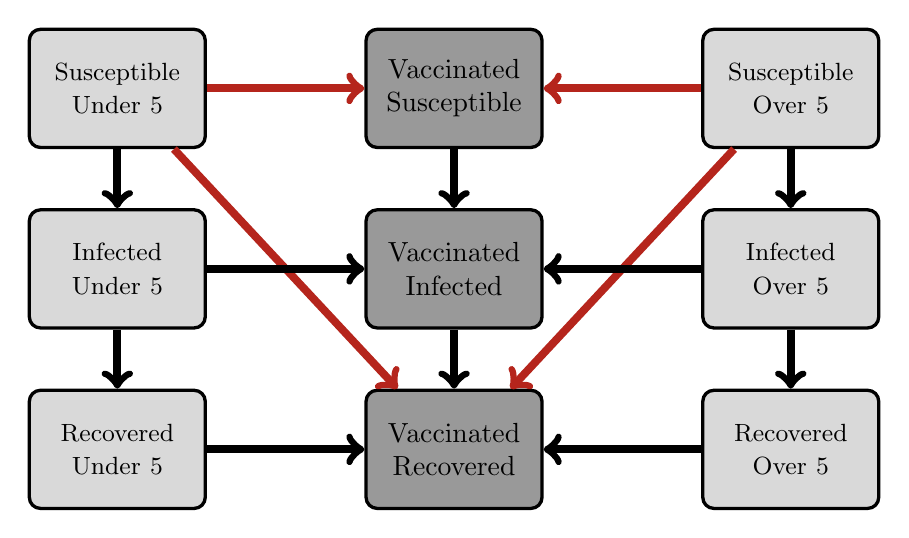
\begin{tikzpicture}
  \node[human node, fill=black!15] (susceptible) {\small Susceptible Under 5};
  \node[human node, fill=black!15,  below=0.75cm of susceptible] (infected) {\small Infected Under 5};
  \node[human node, fill=black!15, below=0.75cm of infected] (recovered) {\small Recovered Under 5};
  
  \node[human node,  right =2cm of susceptible] (susceptiblev) {Vaccinated\\ Susceptible};
  \node[human node,  right=2cm of infected] (infectedv) {Vaccinated Infected};
  \node[human node, right=2cm of recovered] (recoveredv) {Vaccinated Recovered};
  
    \node[human node, fill=black!15, right =2cm of susceptiblev] (susceptibleg5) {\small Susceptible Over 5};
  \node[human node, fill=black!15,  below=0.75cm of susceptibleg5] (infectedg5) {\small Infected Over 5};
  \node[human node, fill=black!15, below=0.75cm of infectedg5] (recoveredg5) {\small Recovered Over 5};
  
  
  
  % the edges
   \draw[normalArrow] (susceptible) -> (infected);
   \draw[normalArrow] (infected)-> (recovered) ;
   
   \draw[normalArrow] (susceptiblev) -> (infectedv);
   \draw[normalArrow] (infectedv)-> (recoveredv) ;
   
   \draw[changedArrow] (susceptible) -> (susceptiblev);
   \draw[changedArrow] (susceptible) -> (recoveredv);
   
   \draw[normalArrow] (infected) -> (infectedv);
   \draw[normalArrow] (recovered) -> (recoveredv);
   
   
    \draw[changedArrow] (susceptibleg5) -> (recoveredv);
    \draw[changedArrow] (susceptibleg5) -> (susceptiblev);
           
    \draw[normalArrow] (susceptibleg5) -> (infectedg5);
    \draw[normalArrow] (infectedg5)-> (recoveredg5) ;
   
    \draw[normalArrow] (infectedg5) -> (infectedv);
   \draw[normalArrow] (recoveredg5) -> (recoveredv);
\end{tikzpicture}

\caption{Model diagram for the DynaMICE model with the population split into three groups:  unvaccinated individuals under the age of 5, unvaccinated individuals over the age of 5, and vaccinated individuals of any age.  Model details are given in \cite{measles}. Red indicates where changes in vaccination policy can be changed to build scenarios.}
\label{fig:MeaslesDiagram}
\end{figure}

\pagebreak

Within this model, $t$ is the time (in years). $S_c /S_a$, $I_c/I_a$, $R_c/R_a$, $VS$, $VI$, $VR$ are the numbers of susceptible, infected, recovered, vaccinated susceptible, vaccinated infected, and vaccinated recovered, within the total population, $N(t)$ which is represented by 

$$N(t) = S_c(t) + S_a(t)+ I_c(t)+I_a(t) + R_c(t) + R_a(t)+VS(t) VI(t) VR(t)$$

The parameters are as follows: $\tau$ is the effectiveness of a single measles vaccine; $\kappa (t)$ is the coverage rate of measles immunization for individuals vaccinated for the first time; $\alpha$ is the birth rate in the population; $\mu$ is the mortality rate and $\gamma$ is the infectiousness period of measles; and $\lambda$ is the rate at which susceptible individuals become infectious upon mutual contact.\\[2ex]


\noindent {\bf Unvaccinated Children Under 5}
\begin{align}
\label{eqn:MeaslesUnder5}
\begin{split}
\frac{dS_{c}}{dt} &= \alpha -\lambda (I_c+I_a+VI) S_c - \mu S_c - \kappa (t) S_c\\
\frac{dI_{c}}{dt} &=\lambda (I_c+I_a+VI) S_c - \mu I_c - \gamma I_c - \kappa(t)I_c\\
\frac{dR_{c}}{dt} &= \gamma I_c - \mu R_c -\kappa (t)R_c\\[3ex]
\end{split}
\end{align}

\noindent {\bf Unvaccinated Adolescents and Adults (Over 5)}
\begin{align}
\label{eqn:MeaslesOver5}
\begin{split}
\frac{dS_{a}}{dt} &= \lambda (I_c+I_a+VI) S_a - \mu S_a - \kappa (t) S_a\\
\frac{dI_{a}}{dt} &=\lambda (I_c+I_a+VI) S_a - \mu I_a - \gamma I_a - \kappa(t)I_a\\
\frac{dR_{a}}{dt} &= \gamma I_a - \mu R_a -\kappa (t)R_a\\[3ex]
\end{split}
\end{align}

\noindent {\bf Vaccinated Individuals (any age)}
\begin{align}
\label{eqn:MeaslesVaccinated}
\begin{split}
\frac{dVS}{dt} &= -\lambda (I_c+I_a+VI)VS - \mu VS + (1-\tau ) \kappa (t) (S_c +  S_a)\\
\frac{dVI}{dt} &= \lambda (I_c+I_a+VI) VS - \mu VI + \kappa (t)(I_c+ I_a) -\gamma VI\\
\frac{dVR}{dt} &= \gamma VI - \mu VR +\tau\kappa (t)(S_c +S_a)+ \kappa (t)(R_c + R_a)
\end{split}
\end{align}

\begin{table}[h!]
\centering
\begin{tabular}{| l | l |}
\hline
Variable & Description \\\hline\hline 
$S_c(t)$ & Susceptible children under the age of 5\\\hline
$I_c(t)$ & Infected children under the age of 5 \\\hline
$R_c(t)$ & Recovered children under the age of 5\\\hline
$S_a(t)$ & Susceptible adolescents and adults over the age of 5\\\hline
$I_a(t)$ & Infected adolescents and adults over the age of 5\\\hline
$R_a(t)$ & Recovered adolescents and adults over the age of 5\\\hline
$VS(t)$ & Susceptible individuals who have been vaccinated\\\hline
$VI(t)$ & Exposed individuals who have been vaccinated\\\hline
$VR(t)$ & Recovered individuals who have been vaccinated\\ \hline
\end{tabular}
\caption{Variable descriptions for the Verguet Measles Model. Further details about initial conditions and parameter values used can be found in the APL-provided code. Further details about the model structure and analysis can be found in \cite{measles}.}
\label{table:MeaslesVariables}
\end{table}

\begin{table}[h!]
\centering
\begin{tabular}{| l | l |}
\hline
Parameter & Description \\\hline\hline 
$\tau$ & Effectiveness of a single measles vaccine\\\hline
$\kappa$ & First-time immunization coverage rate\\\hline
$\alpha$ & Birth rate in the population \\\hline
$\mu$ & Mortality rate in the population\\\hline
$\gamma$ & Infectiousness period of measles\\\hline
$\lambda$ & Rate at which susceptible individuals become infectious upon mutual contact \\\hline
\end{tabular}
\caption{Parameter descriptions for the Verguet measles model. Further details about initial conditions and parameter values used can be found in the APL-provided code. Further details about the model structure and analysis can be found in \cite{measles}.}
\label{table:MeaslesParameters}
\end{table}

\pagebreak

\section{Model Simulation}
\label{sec:Simulations}
Each model was implemented in Python 3.8.  Detailed documentation regarding how to run the models along with the parameter values used to generate the figures below are included in the project github.  The default values are named as follows; 
\begin{itemize}
    \item for cholera,  ``defaultCholeraSimulation.xlsx";
    \item for malaria, ``defaultMalariaSimulation.xlsx"; and,
    \item for measles, ``defaultMeaslesSimulation.xlsx".
\end{itemize}
In general, for each model, initial conditions and parameters values are set via an excel spreadsheet.  This spreadsheet serves as input to the model itself (written in Python).  By default, the output of the model variables is written to a spreadsheet titled according to the disease being simulated (i.e., ``Cholera.xlsx", ``Malaria.xlsx", or ``Measles.xlsx"). Below are sample simulations of each model using their respective default files as input.

\begin{figure}[h!]
    \centering
    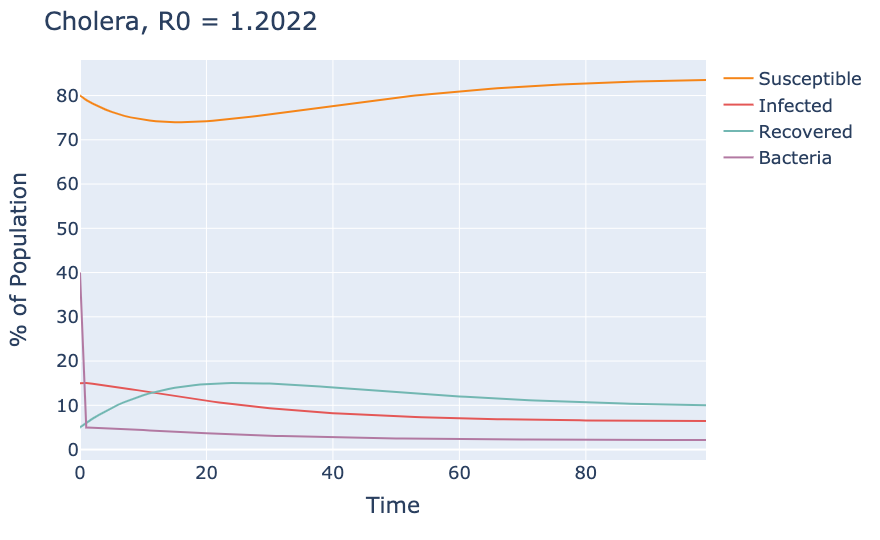
\includegraphics[width = .8\textwidth]{CholeraRun.png}
    \caption{Simulation of the Cholera Model (Equation System (\ref{eqn:choleraEquations})) with initial conditions and parameters given in ``defaultCholeraSimulation.xlsx".}
    \label{fig:my_label}
\end{figure}

\begin{figure}[h!]
    \centering
    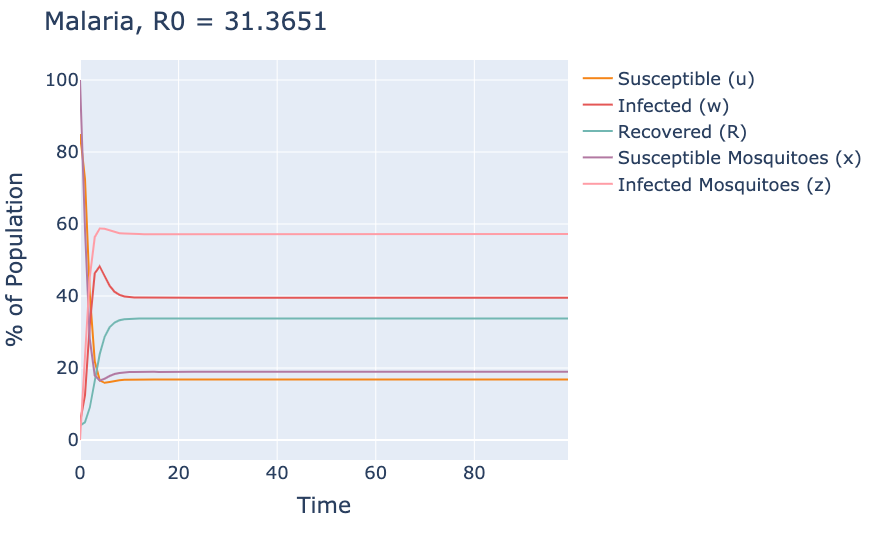
\includegraphics[width = .9\textwidth]{MalariaRun.png}
    \caption{Simulation of the Malaria Model (Equation System (\ref{eqn:malariaEquations}))with initial conditions and parameters given in ``defaultMalariaSimulation.xlsx".}
    \label{fig:my_label}
\end{figure}

\begin{figure}[h!]
    \centering
    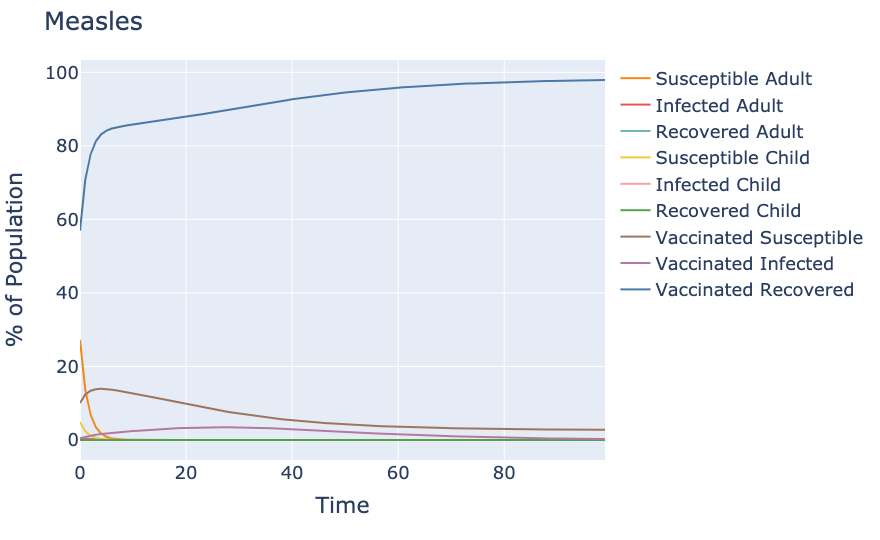
\includegraphics[width = .9\textwidth]{MeaslesRun.png}
    \caption{Simulation of the Measles Model (Equation System (\ref{eqn:MeaslesUnder5} - (\ref{eqn:MeaslesVaccinated})) with initial conditions and parameters given in ``defaultMeaslesSimulation.xlsx".}
    \label{fig:my_label}
\end{figure}

\begin{comment}
\subsubsection{Cholera Model}
\paragraph{Data}

The data on cholera incidence from Dec 2017-Jan 2021 were provided by the Somalia country office of the World Health Organization (WHO).  Data were aggregated to the regional level (Administrative level 1).

\paragraph{Parameters}
Parameters were estimated using the SAEM algorithm \cite{SAEM} in Monolix \cite{monolix}.  The corresponding parameters by region are as follows :

\begin{table}[h!]
    \centering
    {\footnotesize
    \begin{tabular}{|c||c|c| c|c|c| c|c|}
        \hline
         &\multicolumn{7}{c|}{Regions}\\\cline{2-8}
         & Banadir & Gedo & Hiran & Lower Jubba & Middle Shabelle	& Lower  Shabelle & Bay \\\hline\hline	 
         
         $S(0)$ &10.1205&	7.34338&	8.40626&	9.42522&	8.20361&	7.80567&	7.8207\\\hline	 
         
         
        $I(0)$ &316.391	&169.512&	203.392	&311.762&	187.497	&147.275	&182.141\\\hline	 
         
        
        $R(0)$ & 0.241265&	0.0846581&	0.0361393&	0.0403048&	0.035787&	0.0374001&	0.0847241\\\hline	 
         
        $B(0)$ &2.33E+06&	3.37E+06&	1.91E+06&	2.72E+06&	6.87E+06&	669061&	7.44E+07\\\hline	 
         
    $\mu$&	0.0807597&	0.0577582&	0.0660778&	0.0529719&	0.0684865&	0.059394&	0.0445455\\\hline	 
         
    
    $\beta_1$ &	1582&	123.172&	850.048&	393.719&	454.112&	137.95	&210.182\\\hline	 
         
$\beta_2$&	275.467&	41.4836&	111.176&	78.0707&	276.549&	12.4815&	117.352\\\hline
    $\hat{k}$ &\multicolumn{7}{c|}{1E6}\\\hline	 
         
    $\gamma_0$ &\multicolumn{7}{c|}{0.015}\\\hline	 
         
    $\gamma_1$ &\multicolumn{7}{c|}{0.09} \\\hline	 
         
    $\hat{b}$ &\multicolumn{7}{c|}{10}\\\hline	 
         
    $\delta$ &\multicolumn{7}{c|}{30}\\\hline	 
         
    $\alpha$ &\multicolumn{7}{c|}{10}\\\hline

        
    \end{tabular}
    }
    \caption{Parameter values of the Cholera Model when fitted to the case incidences in each region of Somalia.  Parameters are fitted using the SAEM algorithm implemented in Monolix.}
    \label{table:choleraModelValues}
\end{table}

\subsubsection{Malaria Model}
\paragraph{Data} Monthly data on malaria incidence from Jan 2020 - Dec 2020 were provided by the Somalia country office of the World Health Organization (WHO).  This data was reported at the level of zones/states.

\paragraph{Parameters}


\subsubsection{Measles Model}
\paragraph{Data}
The data available related to measles incidence and vaccination rates were unavailable at the time of this report.  As such, the parameters listed below reflect parameters given in \cite{measles}. 

\paragraph{Parameters}
\end{comment}

\section{Future Directions}
\subsection{Somalia Use-Case}
At the time of this report, sub-national infectious disease data was not available for a full parameterization of each of the models. However, upon availability of incidence case data, the model for each infectious disease can be fit according to Section \ref{sec:Parameterization}.


\subsection{Planning Scenarios}
In addition to simulating baseline scenarios, the framework of model implementation allows for the simulation of theoretical scenarios. Scenarios are constructed by changing model parameters at various time points within the simulation. Documentation of how to change model parameters to simulate user-defined scenarios is included in the APL-provided code. Examples of which parameters might be linked with scenario simulations are given below:

\begin{itemize}
    \item {\bf Cholera}
        \begin{itemize}
            \item Adjustments to $\alpha$ might represent changes in water quality such as increased ability to treat the water (decreasing $\alpha$)
            \item Flooding events effect both the quality of water (increasing $\alpha$) as well as increases the rate at which humans interact with contaminated water (increasing $\beta_2$).
            \item Increases and decreases in availability of healthcare facilities are encompassed in the $b$ parameter.
        \end{itemize}
    \item {\bf Malaria}
        \begin{itemize}
            \item Adjusting $\lambda_v$ adjusts the birth-rate of mosquitoes.  For example, this could be adjusted downward in the case of treating public spaces with insecticide or upwards in the case of flooding/excess standing water.  This parameter can also be adjusted seasonally to reflect the seasonal cycle of mosquito prevalence. 
            \item Use of mosquito nets, mosquito spray and other interventions designed to reduce the number of mosquito bites per person can be modeled via adjusting the $\nu_v$ parameter.
            \item Significant increase in the percentage of humans using prophylactics for the prevention of malaria could be simulated by adjusting the $c_{vh}$ parameter downwards.
        \end{itemize}
    \item {\bf Measles}
        \begin{itemize}
            \item The primary factor that might be adjusted is the vaccination rates.  This is adjusted via the $\kappa (t)$ parameter. 
            \item Should a more effective vaccine become available, this would be reflected via changes in the $\tau$ parameter.
        \end{itemize}
\end{itemize}

\subsection{Other Limitations}
It is important to bear in mind that the basic assumptions described in Section \ref{sec:SIR} must be satisfied to produce valid results. As the models are developed independently of one another, joint effects between multiple models are not currently considered. Finally, models for each infectious disease have not been validated with real data, aside from what was completed during model publication by the original authors. As such, additional limitations are unknown, but may be brought to light as models are run using new parameterizations and scenarios.

\subsection{Towards A System Dynamics Model}
Within the context of supporting decision makers, any public health interventions fall short because they are made in piecemeal fashion, rather than from a whole-system perspective. A system dynamics model consists of interlocking sets of differential and algebraic equations [implemented as separate disease models] developed from relevant measured and experiential data \cite{systemsdynamics}.  This work represents the first steps towards the development of a systems dynamics model of infectious diseases.  The current models are implemented independently of each other; however, further development might allow for the the bi-directional linking of these models via other connections with other systems/infrastructure (e.g., health systems, food systems, climate/weather systems).

\clearpage

\begin{thebibliography}{alpha}
\bibitem{basicSIR} Hethcote H. Three Basic Epidemiological Models, pp. 119–144. Berlin, Heidelberg: Springer Berlin, Heidelberg,1989.


\bibitem{systemsdynamics}Homer J., Hirsch G. System dynamics modeling for public health: background and opportunities. Am J Public Health. 2006;96(3):452-458. https://doi.org/doi:10.2105/AJPH.2005.062059.

\bibitem{SAEM} Lavielle, M., Mbogning, C. An improved SAEM algorithm for maximum likelihood estimation in mixtures of non linear mixed effects models. Stat Comput 24, 693–707 (2014). https://doi.org/10.1007/s11222-013-9396-2.

\bibitem{monolix} Monolix version 2019R2. Antony, France: Lixoft SAS, 2021.
http://lixoft.com/products/monolix/.

\bibitem{cholera}Nyabadza, F., Aduamah, J.M. \& Mushanyu, J. Modelling cholera transmission dynamics in the presence of limited resources. BMC Res Notes 12, 475 (2019). https://doi.org/10.1186/s13104-019-4504-9.

\bibitem{malaria} Ngwa, G. \& Shu, W. A mathematical model for endemic malaria with variable human and mosquito populations. Mathematical and Computer Modelling. 32. 747-763 (2000). https://doi.org/10.1016/S0895-7177(00)00169-2. 

\bibitem{measles} Verguet S., Johri M., Morris S., Gauvreau C., Jha P., \& Jit M. Controlling measles using supplemental immunization activities: A mathematical model to inform optimal policy. Vaccine, 33(10). 1291-1296 (2015). https://doi.org/10.1016/j.vaccine.2014.11.050.

\end{thebibliography}

\clearpage

\section{Appendix: Infectious Disease Models Considered}
\label{sec:Appendix}

\begin{enumerate}
\item Grad, Y.H., Miller, J.C., and Lipsitch M. Cholera Modeling: Challenges to Quanititative Analysis and Predicting the Impact of Intercentions. Epidemiology, 23(4). 523-530 (2012 Jul). https://doi.org/10.1097/EDE.0b013e3182572581. \\
\item Chao, D.L., Longini, I.M., and Morris, J.G. Modeling cholera outbreaks. Curr Top Microbiol Immunol, 379. 195-209 (2014). https://doi.org/10.1007/82\underscore2013\underscore307. \\
\item Sun, G.Q., Xie J.H., Huang, S.H., Jin Z., Li M.T., Liu L. Transmission dynamics of cholera: Mathematical modeling and control strategies. Communications in Nonlinear Science and Numerical Simulation, 45. 235-244 (2017 Apr). https://doi.org/10.1016/j.cnsns.2016.10.007. \\
\item Cui J., Wu Z., and Zhou X. Mathematical Analysis of a Cholera Model with Vaccination. Journal of Applied Mathematics, vol. 2014. (2014). https://doi.org/10.1155/2014/324767. \\
\item Bakary T., Boureima S., and Sado T. A mathematical model of malaria transmission in a periodic environment. Journal of Biological Dynamics, 12(1). 400-432 (2018). https://doi.org/10.1080/17513758.2018.1468935. \\
\end{enumerate}



\end{document}